\documentclass{article}

% ML4PS 2026 submission 10. Reconstructed from the submitted PDF (11 September 2026);
% the source of that build was not kept. Build: tectonic -X compile main.tex
\usepackage[final]{neurips_2026}

\usepackage[utf8]{inputenc}
\usepackage[T1]{fontenc}
\usepackage{hyperref}
\usepackage{url}
\usepackage{booktabs}
\usepackage{amsfonts}
\usepackage{nicefrac}
\usepackage{microtype}
\usepackage{xcolor}
\usepackage{graphicx}

\title{Did your model learn the physics or the simulator?\\Intervening on a generative process, one ingredient at a time}

\author{%
  Owen Yang\\
  Henry M.\ Gunn High School\\
  780 Arastradero Rd, Palo Alto, CA 94306, USA\\
  \texttt{owenhyang@gmail.com}\\
}

\begin{document}

\maketitle

\begin{abstract}
Training on simulator output is the shared condition of most machine learning for the physical sciences, and it raises a question the usual robustness report does not answer: how much of what the model learned is the phenomenon, and how much is the simulator? We intervene on the generative process itself---changing one ingredient of the physics and re-rendering the same 9,072 objects, or perturbing their observation---rather than corrupting fixed inputs. The testbed is exoplanet transmission spectra at the configuration ESA's Ariel mission \citep{tinetti2018} will deliver---where machine-learning screens over simulated spectra are actively proposed \citep{marquezneila2018,duquecastano2025,yip2023}---but every finding is about simulator-trained models. On transferability: across a balanced grid of two model families crossed with three representations, the ordering of the losses transfers, and the representation carries it---pipelines sharing a representation agree at mean Spearman $\rho = 0.94$ against 0.85 for every other pair ($p = 0.009$), while sharing a model family agrees no better than sharing nothing. Magnitudes do not transfer: the same shift costs a median $8\times$ more for one pipeline than another, and the ranking inverts under strong shift, with the pipeline 6.4 points worse in-domain becoming 16 points better under heavy haze. On repair: shifts described by a handful of numbers---contamination, haze, an instrument ramp---are 79--89\% recoverable by augmentation for 1.4 points of clean accuracy, whereas noise drawn afresh in every bin, at equal cost, is only 29--35\% recoverable; a model can learn a transformation but not a particular draw. On the audit: the approximations the model notices are not the ones a modeler checks. The radiative-transfer implementation costs 2.4 points, the observing environment 26. Data, paired re-renders, and code are released.
\end{abstract}

\section{Introduction}

A model trained on simulator output has learned two things at once: the phenomenon the simulator represents, and the simulator's own approximations. Which is which is rarely asked, and the usual robustness report---accuracy falls by $x$ under shift---does not separate them. It matters because the second part is under the practitioner's control: some simulator errors can be modeled away, some trained away, and some neither, and knowing which is which decides where finite effort goes.

Robustness benchmarks largely apply synthetic corruptions---blur, noise, compression---to fixed inputs \citep{hendrycks2019}, and robustness so measured does not transfer to natural shift, where clean accuracy predicts shifted accuracy along a trend few interventions beat \citep{taori2020}; calibration degrades faster than accuracy \citep{ovadia2019}, and simulation-trained astronomical models degrade similarly \citep{ciprijanovic2021}. Simulation-based inference asks the nearest question \citep{cranmer2020}, and the effect of a misspecified simulator on a trained posterior has been measured directly \citep{cannon2022}, though never as a budget over named ingredients. Our shifts are \emph{interventions on the generative process}: we change one ingredient of the physics---the radiative-transfer code, a molecular line list, the presence of aerosols or stellar activity---and re-render the same planets, so each cost is a within-planet difference attributable to a named modeling decision.

Three sub-questions make that separation measurable: which of the simulator's approximations the model actually notices, as opposed to those its authors worry about; which of the resulting losses can be trained away; and whether the answer describes the task or only the pipeline that produced it. Sections~3 to~5 take the three questions in turn. The last of them has been asked of a single accuracy number \citep{taori2020}; Section~5 asks it of the whole ordering, on a grid balanced so that the representation separates from the model family, which to our knowledge is new. The paired re-renders behind all of it are released.\footnote{Repository: \url{https://github.com/oy2017/BioSignatureDetectionModel}, branch \texttt{ml4ps-benchmark}.}

\section{Setup}

\textbf{Data.} H$_2$-dominated transmission spectra are simulated with MultiREx \citep{duquecastano2025} over TauREx~3 \citep{alrefaie2021}. The grid has 15 parameters; all but the two label gases are drawn independently (max $|r| = 0.07$), which makes each sensitivity attributable but leaves the grid a stress-test box. The two label gases are stratified instead: half the planets biosignature-bearing, the rest split equally between CH$_4$-only, O$_3$-only and neither. That balances the classes and puts two-thirds of the negatives in the two confusable one-gas cases, at $r = +0.18$ within the pair and $|r| < 0.02$ elsewhere. Spectra are computed once, noise-free, at $R \approx 1000$, then binned to the layout Ariel delivers for its deepest tier---three photometric bands below 1.1~$\mu$m, then $R = 15, 100, 30$ across 1.1--7.8~$\mu$m, 102 bins---with per-bin noise shaped by an ExoRad~2 \citep{mugnai2023} model of the payload. After cleaning: 18,156 training and $5 \times {\sim}1{,}815$ test spectra.

\textbf{Label.} Positive iff $\log X_{\mathrm{CH_4}} > -6$ and $\log X_{\mathrm{O_3}} > -7$, a deterministic function of the injected abundances. The task is recovery of a labeling convention, not detection: the chemistry is a vehicle, and in a hot H$_2$ atmosphere ozone at these abundances is thermochemically forbidden anyway. Classes are balanced: every accuracy is at a 1:1 prior.

\textbf{Pipeline.} The audited pipeline, frozen below, is gradient-boosted trees on per-spectrum normalized bins, tuned by five-fold cross-validation and refitted only where augmentation is the experiment. Section~5 scores five others on the identical data.

\textbf{Shift protocol.} Four axes re-render the same planets from their recorded parameters with one ingredient changed: an independent radiative-transfer code (Exo-Transmit \citep{kempton2017}, opacities fixed), alternative opacities (ExoMolOP \citep{chubb2021}, and a variant also replacing ozone), cloud decks and Mie hazes \citep{lee2013}, and stellar contamination via the transit light source effect \citep{rackham2018} with PHOENIX spectra \citep{allard2012}. Two perturb the clean spectra: noise, white or spectrally correlated, and instrument systematics, multiplicative or additive. A seventh axis instead restricts the training grid in planet radius and tests outside it. Each axis is rendered at several strengths, giving 48 shifted cases. Noise uses the clean spectrum's level and the planet's own seed, so a suppressed atmosphere is not given less noise.

\section{Which approximations does the model notice?}

Table~\ref{tab:budget} and Figure~\ref{fig:main}A give the fidelity budget: the loss under each change, paired per planet against the clean 90.33\% baseline. Because the same planets carry every change, each cost isolates how much of the model's accuracy depended on one named simulator choice rather than on the phenomenon it stands for. \emph{Implementation choices are nearly free until they touch the label}: an independent RT code costs 2.4 points, the classifier-level price of a ppm-level disagreement between retrieval codes \citep{barstow2020}, and alternative line lists for the three non-label gases cost 1.7 points, but swapping the line list of a label-bearing gas costs 15.5 points and moves the predicted-positive rate from 0.50 to 0.34---a displaced boundary, not lost signal \citep{niraula2022}. \emph{Changing spectral shape costs most}: a haze costs 28.8 points while leaving 76\% of the feature amplitude, against 11.6 for a cloud deck leaving 67\%, the haze imposing a wavelength-dependent slope where the deck dims uniformly. Coverage is separate, sitting between those extremes: testing outside the training envelope in planet radius costs 6.2 points against a matched control, a known failure mode for supervised retrieval \citep{nixon2020}.

\begin{table}[t]
  \caption{Fidelity budget: accuracy change of the frozen pipeline on the same 9,072 test planets, paired per planet, against a clean baseline of 90.33\%. Amplitude is the median noise-free feature amplitude relative to clean.}
  \label{tab:budget}
  \centering
  \small
  \begin{tabular}{lrrr}
    \toprule
    Change & $\Delta$ acc. & pred. pos. rate & amplitude \\
    \midrule
    Independent RT code (Exo-Transmit) & $-2.4$ & 0.49 & 0.89 \\
    Alternative opacities, 3 non-label gases & $-1.7$ & 0.54 & 0.92 \\
    \quad and the label-bearing (O$_3$) line list too & $-15.5$ & 0.34 & 0.86 \\
    Haze, $3 \times 10^{7}$~m$^{-3}$ & $-28.8$ & 0.12 & 0.76 \\
    Cloud deck, $10^{3}$~Pa & $-11.6$ & 0.33 & 0.67 \\
    Stellar spots, 20\% coverage (stress) & $-25.9$ & 0.16 & 1.05 \\
    Global additive offset, $2\times$ noise & $0.0$ & 0.50 & 1.00 \\
    Per-channel additive offsets, $2\times$ noise & $-10.6$ & 0.44 & 1.00 \\
    \bottomrule
  \end{tabular}
\end{table}

\section{Which of those can be trained away?}

We retrain with the shift randomized over the training set \citep{tobin2017}---each planet at a random strength, a third left clean---and score on the identical shifted test planets.

\begin{center}
  \small
  \begin{tabular}{llrr}
    \toprule
    Shift (axis, strengths) & kind & frozen $\to$ augmented & gap recovered \\
    \midrule
    Stellar spots, 5--20\% coverage & deterministic & 79.7--64.4 $\to$ 88.1--85.3\% & 79--83\% \\
    Haze, $2 \times 10^{6}$--$2.4 \times 10^{8}$~m$^{-3}$ & deterministic & 82.6--52.5 $\to$ 88.8--84.0\% & 80--89\% \\
    Gain ramp, $2\times$ noise & deterministic up to a sign & 82.4 $\to$ 89.0\% & 84\% \\
    Correlated noise, SNR 10--5 & stochastic & 84.0--69.0 $\to$ 86.0--75.6\% & 31--35\% \\
    White noise, SNR 5 & stochastic & 77.5 $\to$ 81.1\% & 29\% \\
    \bottomrule
  \end{tabular}
\end{center}

Only cases costing the frozen pipeline over 5 points are included, since the recovered fraction is unstable at small denominators. On that criterion the split does not overlap: 79--89\% across seven deterministic cases against 29--35\% across four stochastic ones.

The separating property is not how much signal is lost---the strongest haze removes 40\% of the feature amplitude and is still 83\% recoverable---but how many numbers the shift draws for each spectrum. Contamination and haze are fixed by the contaminant, so a model shown examples learns an approximate inverse; noise is drawn afresh in every bin, and augmentation teaches its distribution but cannot undo a realization. Contamination, haze and the two noise axes would on their own confound this with physics, since both of the repairable ones are re-renders. The gain ramp breaks that confound: an instrument systematic injected exactly as the noise is, whose whole effect on a spectrum is one tilt and a sign drawn per planet. It repairs at 84\%, so a single drawn bit is no obstacle where a draw per bin is fatal. Frequency content does not order the split either: the correlated noise is the smoothest of the five, 2\% of its power above an eighth of a cycle per bin against the haze's 11\%, and it repairs worst \citep{yin2019}.

The rule is checkable before any experiment, but the obvious way to measure it fails: a learned inverse map back to the clean spectrum recovers as much variance on the stochastic axes as on the deterministic ones (0.73--0.91 against 0.74--0.77), so it does not rank repairability. The rule is also established post hoc; whether it predicts on unseen shifts is untested.

\section{What carries the budget: the representation, not the model}

An audit like Section~3 is only reusable if it describes the task. We repeat every shift on a balanced grid---two model families (XGBoost, random forest) crossed with three representations (per-spectrum normalized, PCA scores, raw bins). Across the 48 cases the ordering is broadly stable, and not trivially so: ranking the shifts by surviving feature amplitude, a physical proxy, gives only $\rho = 0.39$.

\begin{figure}[t]
  \centering
  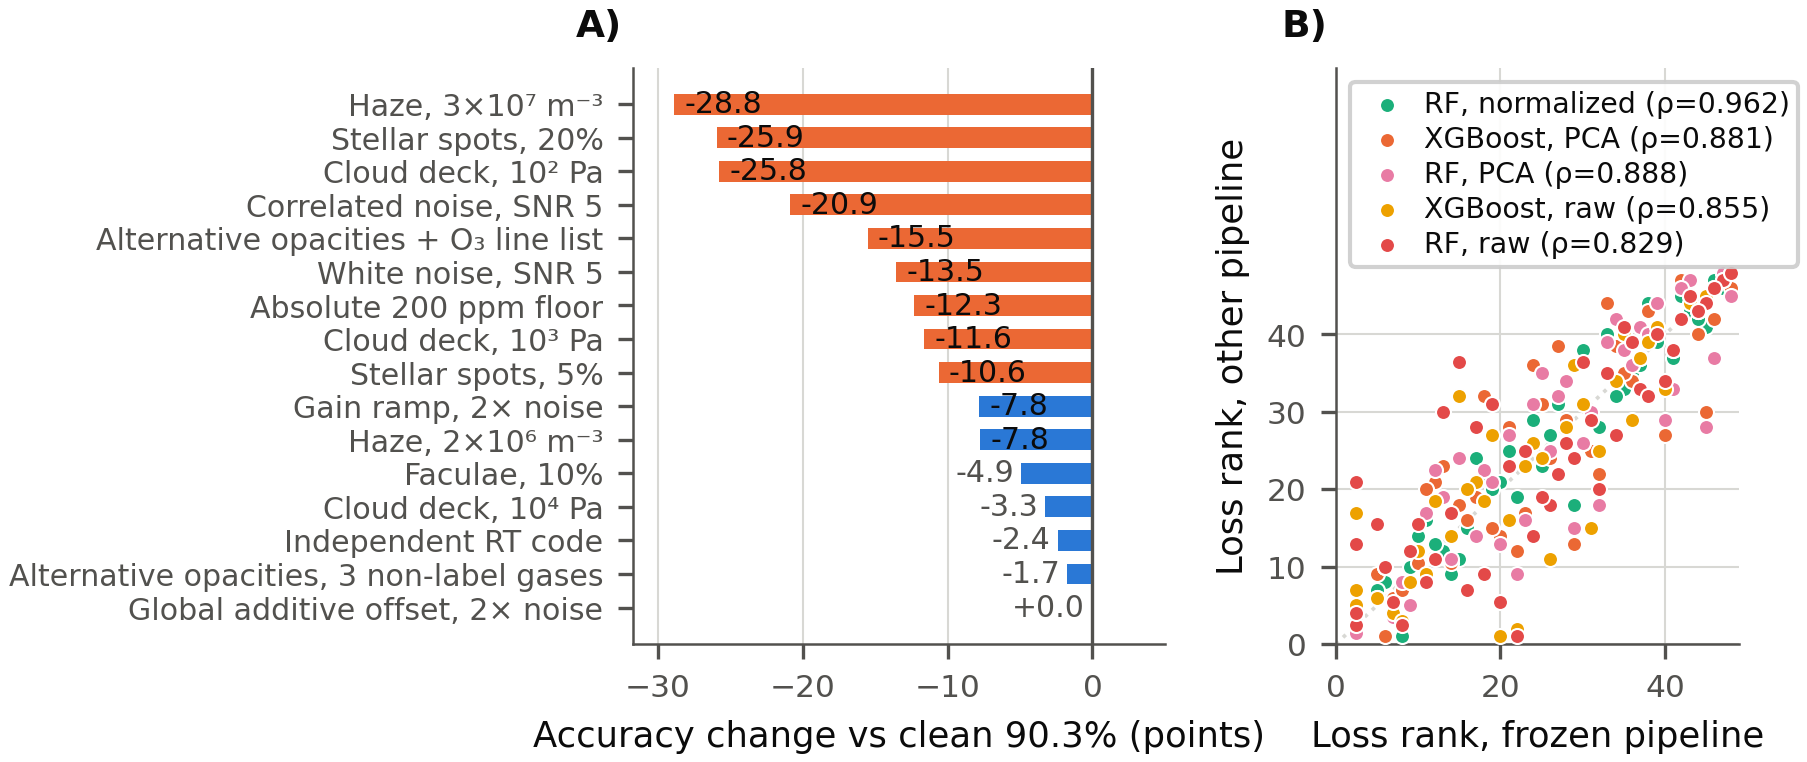
\includegraphics[width=\linewidth]{figures/budget.png}
  \caption{A) Fidelity budget for the frozen pipeline: accuracy change on the same test planets under each single-ingredient change (orange, $|\Delta| \geq 10$ points). B) All 48 cases scored with five further pipelines, ranked by loss against the frozen pipeline's ranking; $\rho$ is the Spearman correlation, and RF is random forest.}
  \label{fig:main}
\end{figure}

The 15 pipeline pairs separate by what they share. Pairs sharing a representation agree at mean $\rho = 0.944$; pairs sharing a model family agree at 0.846, which is identical to the agreement of pairs sharing neither (0.846). Sharing a model family buys nothing; sharing a representation closes about two-thirds of the gap left to perfect agreement (one-sided Mann--Whitney $p = 0.009$; $p = 0.024$ against the family-sharing pairs alone). The ranges overlap once, so this is a difference in means, not a clean partition.

Magnitudes are another matter: across the 28 cases costing any pipeline over 5 points, the same shift costs a median $8\times$ more for one pipeline than another, and the ranking inverts. Under a haze at $3 \times 10^{7}$~m$^{-3}$ the frozen pipeline falls to 61.5\% while the PCA pipeline---6.4 points worse in-domain---holds 77.8\%. This is not a floor effect: raw bins start 17.8 points lower still and fall to 59.6\%, below the frozen pipeline, so lower clean accuracy does not buy robustness. The inversion appears at $\geq 5\%$ spot coverage and at $10^{2}$~Pa decks, and not at weaker shifts. Weighted over a population, switching pipelines only pays above about 28\% prevalence of severe haze. The usable conclusion is narrow: borrow a published budget as a ranking, never as numbers.

The same asymmetry appears in-domain: across the same grid plus an MLP, the spread over representations is an order of magnitude larger than that over models. Per-spectrum normalization, the standard normal variate of chemometrics \citep{barnes1989}, takes XGBoost from 72.6\% on raw bins and 83.9\% on PCA scores to $90.3 \pm 0.4\%$; with it that model, a random forest and an MLP lie within 1.3 points and the top two are statistically tied (McNemar $p = 0.36$). A logistic regression on the same features reaches $85.4 \pm 0.4\%$, putting the nonlinear model at 5.0 points against the representation's 17.8---raw bins to normalized, same model. What survives is spectral shape, which sets the failure mode: the global offset in Table~\ref{tab:budget} costs nothing by construction, while the per-channel offsets a six-channel payload actually produces cost 10.6 points at twice the noise level.

\section{Conclusion and limitations}

A loss profile is useful to a reader with a different model only if it transfers. This one does, as a ranking carried by the representation: sharing a representation buys the agreement, sharing a model family buys none. The losses do split cleanly by one thing: how many numbers the shift draws per spectrum, which sets what augmentation buys, 79--89\% against 29--35\%. Beyond the stress-test grid already noted, atmospheres are isothermal and pure H$_2$: collision-induced absorption is absent, and isothermality alone biases retrieved abundances by about a decade \citep{rocchetto2016}; no axis tests either of them. The haze is uniformly mixed, which makes its rows upper bounds, and every figure assumes a 1:1 prior no survey will have.

\small
\begin{thebibliography}{99}
\bibitem[Tinetti et al.(2018)]{tinetti2018} Tinetti, G., et al. (2018). A chemical survey of exoplanets with ARIEL. \emph{Exp. Astron.}, 46(1), 135--209.
\bibitem[Márquez-Neila et al.(2018)]{marquezneila2018} Márquez-Neila, P., Fisher, C., Sznitman, R., \& Heng, K. (2018). Supervised machine learning for analysing spectra of exoplanetary atmospheres. \emph{Nat. Astron.}, 2(9), 719--724.
\bibitem[Duque-Castaño et al.(2025)]{duquecastano2025} Duque-Castaño, D. S., Zuluaga, J. I., \& Flor-Torres, L. (2025). Machine-assisted classification of potential biosignatures in Earth-like exoplanets using low signal-to-noise ratio transmission spectra. \emph{MNRAS}, 539(2), 1528--1552.
\bibitem[Yip et al.(2023)]{yip2023} Yip, K. H., Changeat, Q., Al-Refaie, A., \& Waldmann, I. P. (2023). Lessons learned from the Ariel Data Challenge 2022. \emph{PMLR}, 220, 1--17.
\bibitem[Hendrycks \& Dietterich(2019)]{hendrycks2019} Hendrycks, D., \& Dietterich, T. (2019). Benchmarking neural network robustness to common corruptions and perturbations. \emph{ICLR}.
\bibitem[Taori et al.(2020)]{taori2020} Taori, R., Dave, A., Shankar, V., Carlini, N., Recht, B., \& Schmidt, L. (2020). Measuring robustness to natural distribution shifts in image classification. \emph{NeurIPS}, 33.
\bibitem[Ovadia et al.(2019)]{ovadia2019} Ovadia, Y., et al. (2019). Can you trust your model's uncertainty? Evaluating predictive uncertainty under dataset shift. \emph{NeurIPS}, 32.
\bibitem[Ćiprijanović et al.(2021)]{ciprijanovic2021} Ćiprijanović, A., et al. (2021). DeepMerge -- II. Building robust deep learning algorithms for merging galaxy identification across domains. \emph{MNRAS}, 506(1), 677--691.
\bibitem[Cranmer et al.(2020)]{cranmer2020} Cranmer, K., Brehmer, J., \& Louppe, G. (2020). The frontier of simulation-based inference. \emph{PNAS}, 117(48), 30055--30062.
\bibitem[Cannon et al.(2022)]{cannon2022} Cannon, P., Ward, D., \& Schmon, S. M. (2022). Investigating the impact of model misspecification in neural simulation-based inference. \emph{arXiv:2209.01845}.
\bibitem[Al-Refaie et al.(2021)]{alrefaie2021} Al-Refaie, A. F., Changeat, Q., Waldmann, I. P., \& Tinetti, G. (2021). TauREx 3: A fast, dynamic, and extendable framework for retrievals. \emph{ApJ}, 917(1), 37.
\bibitem[Mugnai et al.(2023)]{mugnai2023} Mugnai, L. V., Bocchieri, A., \& Pascale, E. (2023). ExoRad 2.0: The generic point source radiometric model. \emph{JOSS}, 8(89), 5348.
\bibitem[Kempton et al.(2017)]{kempton2017} Kempton, E. M.-R., Lupu, R., Owusu-Asare, A., Slough, P., \& Cale, B. (2017). Exo-Transmit: An open-source code for calculating transmission spectra for exoplanet atmospheres of varied composition. \emph{PASP}, 129(974), 044402.
\bibitem[Chubb et al.(2021)]{chubb2021} Chubb, K. L., et al. (2021). The ExoMolOP database: Cross sections and k-tables for molecules of interest in high-temperature exoplanet atmospheres. \emph{A\&A}, 646, A21.
\bibitem[Lee et al.(2013)]{lee2013} Lee, J.-M., Heng, K., \& Irwin, P. G. J. (2013). Atmospheric retrieval analysis of the directly imaged exoplanet HR 8799b. \emph{ApJ}, 778(2), 97.
\bibitem[Rackham et al.(2018)]{rackham2018} Rackham, B. V., Apai, D., \& Giampapa, M. S. (2018). The transit light source effect: False spectral features and incorrect densities for M-dwarf transiting planets. \emph{ApJ}, 853(2), 122.
\bibitem[Allard et al.(2012)]{allard2012} Allard, F., Homeier, D., \& Freytag, B. (2012). Models of very-low-mass stars, brown dwarfs and exoplanets. \emph{Phil. Trans. R. Soc. A}, 370(1968), 2765--2777.
\bibitem[Barstow et al.(2020)]{barstow2020} Barstow, J. K., Changeat, Q., Garland, R., Line, M. R., Rocchetto, M., \& Waldmann, I. P. (2020). A comparison of exoplanet spectroscopic retrieval tools. \emph{MNRAS}, 493(4), 4884--4909.
\bibitem[Niraula et al.(2022)]{niraula2022} Niraula, P., de Wit, J., Gordon, I. E., Hargreaves, R. J., Sousa-Silva, C., \& Kochanov, R. (2022). The impending opacity challenge in exoplanet atmospheric characterization. \emph{Nat. Astron.}, 6, 1287--1295.
\bibitem[Nixon \& Madhusudhan(2020)]{nixon2020} Nixon, M. C., \& Madhusudhan, N. (2020). Assessment of supervised machine learning for atmospheric retrieval of exoplanets. \emph{MNRAS}, 496(1), 269--281.
\bibitem[Tobin et al.(2017)]{tobin2017} Tobin, J., Fong, R., Ray, A., Schneider, J., Zaremba, W., \& Abbeel, P. (2017). Domain randomization for transferring deep neural networks from simulation to the real world. \emph{IROS}, 23--30.
\bibitem[Yin et al.(2019)]{yin2019} Yin, D., Gontijo Lopes, R., Shlens, J., Cubuk, E. D., \& Gilmer, J. (2019). A Fourier perspective on model robustness in computer vision. \emph{NeurIPS}, 32.
\bibitem[Barnes et al.(1989)]{barnes1989} Barnes, R. J., Dhanoa, M. S., \& Lister, S. J. (1989). Standard normal variate transformation and de-trending of near-infrared diffuse reflectance spectra. \emph{Appl. Spectrosc.}, 43(5), 772--777.
\bibitem[Rocchetto et al.(2016)]{rocchetto2016} Rocchetto, M., Waldmann, I. P., Venot, O., Lagage, P.-O., \& Tinetti, G. (2016). Exploring biases of atmospheric retrievals in simulated JWST transmission spectra of hot Jupiters. \emph{ApJ}, 833(1), 120.
\end{thebibliography}

\end{document}
